\chapter{Active Matter Systems}
\label{ch:activeandpassivemattersystems}

\section{Fundamentals of Active Matter}
\label{sct:fundamentalsofactivematter}

%====================================================================== New paragraph

The definition of active matter is not always the same across the literature. Some authors describe it in a broad way, emphasizing that the key element is the continuous intake and dissipation of energy by each unit, which allows them to remain out of equilibrium and sustain motion or internal stresses. Reviews often highlight internally driven systems—such as cytoskeletal extracts, swimming microorganisms, or synthetic colloids—as the most representative examples of active matter~\cite{ramaswamy2010mechanics, marchetti2013hydrodynamics, bechinger2016active}.

Other authors focus more specifically on self-propulsion at the particle level as the defining feature. This perspective is useful for distinguishing active systems from those whose dynamics are mainly caused by externally imposed forces. For example, in vibrated granular monolayers, asymmetric grains can display self-propelled trajectories and flock-like patterns and are sometimes described as active. In contrast, symmetric grains that only move in a directed way because of an asymmetric boundary, such as a sawtooth channel, are better classified as externally driven rather than active~\cite{deseigne2010collective, mobarakabadi2013granular, fernandez2022active}.

There is also a difference when considering individual vs. collective behavior. Some colloids appear passive when studied alone, but when interactions are taken into account, they can exhibit genuinely non-equilibrium collective phenomena. Examples include motility-induced phase separation (MIPS), defect-mediated flows in active nematics, and other emergent patterns normally linked with active matter. For this reason, several reviews describe active matter not only in terms of single-particle propulsion but also in terms of its collective stresses and patterns~\cite{cates2015motility, doostmohammadi2018active}.

Simple theoretical models have played a crucial role in understanding active matter. One of the best-known examples is the Vicsek model, which shows how local alignment rules together with noise can lead to large-scale collective motion from basic self-driven units~\cite{vicsek1995novel, chate2008collective}. At the level of single particles, the Active Brownian Particle model is a common way to study colloidal swimmers. In this model, motion is explained by a constant propulsion force, combined with random changes in orientation resulting from rotational diffusion~\cite{romanczuk2012active, elgeti2015physics}.


More recent works point out that definitions have evolved over time and suggest clarifying criteria such as whether the drive is internal or external, whether the system is dry or wet (momentum non-conserving or conserving), and whether the energy input acts at the particle level. Some surveys even propose that researchers explicitly state their working definition depending on the context of their problem~\cite{gompper20202020, gompper20252025}.

\paragraph{Working definition.} In this thesis, we define active matter as:
\begin{quote}
systems composed of units that continuously draw energy at the particle scale and convert it into mechanical work, generating persistent stresses or self-propulsion, and sustaining non-equilibrium collective dynamics.
\end{quote}

This definition includes both biological and synthetic systems (such as bacteria, cytoskeletal extracts, and Janus colloids) but excludes setups where directed motion arises only from externally imposed vibrations or asymmetric boundaries without particle-level energy input—for example, symmetric grains transported by a sawtooth channel~\cite{reimann2002brownian, hanggi2009artificial}.



We will first present some macroscopic examples that show universal principles of self-organization, and then move to the microscopic cases most relevant to this work—active colloids, run-and-tumble swimmers, and active nematics—where thermal noise and low-Reynolds-number hydrodynamics play a dominant role.

%========================================================================

\section{Macroscopic Agents}

Examples of active matter can be observed at plain sight in the macroscopic world. A flock of birds, for instance, is considered active matter because each bird is capable of self-propulsion. Unlike microscopic systems, they are not significantly affected by the thermal noise of their medium—in this case, air. A computational study by Reynolds (1987) modeled flocking behavior in birds by treating each individual as an autonomous agent whose trajectory was influenced by its local environment and neighboring individuals~\cite{reynolds1987flocks}.

Reynolds introduced three fundamental rules governing flocking behavior: separation (collision avoidance), alignment (velocity matching with neighbors), and cohesion (attraction toward the average position of neighbors). This work laid the foundation for understanding how simple local interactions can give rise to complex patterns of collective motion. 

Over time, further developments in the study of group dynamics have incorporated methods such as dynamical maximum entropy to predict the alignment of ordered groups~\cite{cavagna2014dynamical}. Following a maximum entropy approach, network reshuffling was later studied~\cite{mora1511questioning}. These behaviors, however, can change due to external factors, such as predation risk, which influences the formation and density of flocks~\cite{carere2009aerial}. In addition, individual characteristics can also affect collective behavior~\cite{couzin2002collective}.


There are also self-organized groups of smaller flying animals whose collective behavior is even more complex than that of larger species. For example, bees are capable of dividing labor as a result of social interactions among individuals~\cite{jeanson2005emergence}. Remaining within the field of insects but shifting to a solid medium, ants exhibit similar patterns of labor division. Their organization can transition between ordered and disordered states depending on colony size. The disordered state typically occurs when the number of foraging ants is small, due to the infrequent discovery of food~\cite{beekman2001phase}. However, even when the colony is large enough to sustain a greater number of foragers, problems can still arise. In particular, some ants may remain stationary, occupying tunnels and thereby reducing the overall flow rate~\cite{aguilar2018collective}.

\begin{figure}
  \begin{center}
    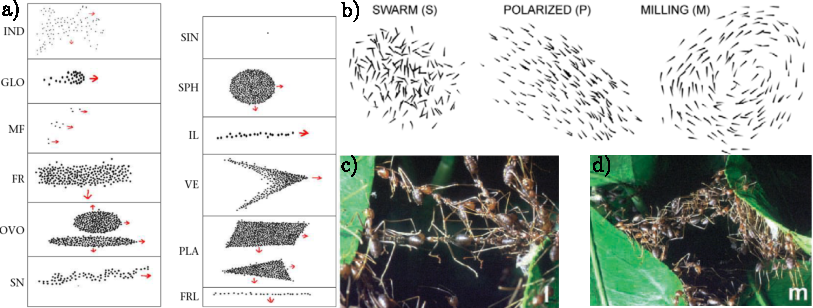
\includegraphics[width=0.95\textwidth]{figures/macroscopicagents.pdf}
  \end{center}
  \caption[Macroscopic Agents example]{\textbf{Panel 1)} Example of different formation of birds deppending predation risk, obtained from~\cite{carere2009aerial}. \textbf{Panel 2)} Different formation of schooling fish, obtained from~\cite{tunstrom2013collective}. \textbf{Panel 3) - 4)} Aggregation of ants forming a bridge, obtained from~\cite{anderson2002self}.}\label{fig:macroscopicagents}
\end{figure}


Another characteristic that arises from self-organization in ants—one not possessed by all animals—is their ability to self-assemble to perform specific tasks. Examples include the formation of rafts, bridges, or columns, where each individual uses its legs or jaws to grasp another and remains in place until the collective goal is achieved. Naturally, certain factors influence these self-assemblages, one of the most significant being colony size~\cite{anderson2002self}. Interesntingly, these structures posses some viscoelastic properties, when applied a certain stress, they tend to return to their original place, resulting in an elastic behavior, at the same time they adapt a viscous behavior due to objects being able to sink in the aggreagation, the same way they would do in a viscous fluid~\cite{tennenbaum2016mechanics}. This opens the posibility for ants to be used as smart materials. 

There are also animals that form groups while inhabiting more complex environments, such as water. Regardless of the medium, different species often display similar behaviors and dependencies. For example, the dynamics of schooling fish can be predicted, typically resulting in three main configurations, with variations depending on group size~\cite{tunstrom2013collective, katz2011inferring, huang2024collective}.

These are just few examples of large animal groups that, interestingly, share common characteristics of self-organization. This process begins at the level of the individual but emerges as a collective, temporary order through direct or indirect interactions among organisms, ultimately allowing them to achieve a common goal~\cite{isaeva2012self}.

The study of macroscopic agents reveals that self-organization is not limited to large animal groups. At smaller scales, microscopic agents such as bacteria, colloidal particles, and artificial swimmers also exhibit analogous self-organized behaviors, although these are driven by different physical principles, including thermal noise and low-Reynolds-number hydrodynamics.

\section{Microscopic agents}

As discussed in the previous section, the term active matter is not limited to microscopic systems but also applies to animal groups. However, the focus of this thesis will be on the former.

We have already defined how a passive brownian particle acts, therefore let us review the key difference of active and passive ones. Passive particles undergo mere diffusion motion, whereas active follows stochastic differential equations accordnig to~\cite{volpe2014simulation}:

\begin{align}
  \frac{d}{dt}x(t) &= v\cos{\varphi(t)} + \sqrt{2D_T}W_x,\\
  \frac{d}{dt}y(t) &= v\sin{\varphi(t)} + \sqrt{2D_T}W_y,
  \label{eq:activestochasticequation}
\end{align}

where $W_x$, and $W_y$ represent their corresponding Wiener process, and \textit{v} is the mean velocity. As stated before, if 

\begin{equation}
  \lim_{v \to 0}  v\cos{\varphi(t)} + \sqrt{2D_T}W_x,
  \label{eq:limitofvelocity}
\end{equation}

then the motion is merely diffusive and the particle is characterized as passive brownian particle. 

However, they also exhibit some randomness; it is rare for them to move exactly in a straight line, and this is where chirality comes into play. There are three different forms of asymmetry: rotational, reflexional, and a combination of the two. If a particle does not meet any of the three criteria, then the particle is not symmetric in any aspect. Chirality is actually the name for a non-reflexive-symmetric particle, as exemplified by our hands, from which the actual word originates~\cite{cahn1966specification}.

Therefore adding an important third term for the rotational diffusion given by:

\begin{equation}
  \frac{d}{dt}{\varphi} = \sqrt{2D_R}W _{\varphi}.
  \label{eq:rotationaldiffusion}
\end{equation}


Despite this limitations, researchers have been developing new methods to achieve self-propulsion that mimic natural processes. In the following subsections, we will introduce a few examples of different systems that have been created, as well as organic ones.


\subsection{Artificial Systems}

As discussed in Section~\ref{sct:fundamentalsofactivematter}, the definition encompasses various mechanisms of self-propulsion, and the list and discoveries are extensive.

Take, for example, \textit{PDMS platelets coated with Pt} by Ismagilov et al. (2002), it appears to be the first realization of this method. The motion itself is not performed by the particle, but by the layer of platinum (catalyst). This is a chemical reaction where the components move by the releasing of bubbles produced when a liquid (hydrogen peroxide) breaks down with the help of a catalyst~\cite{ismagilov2002autonomous}. If we examine the definition of a catalyst, this one does not seem to be affected by the reaction; therefore, the movement would occur indefinitely. In fact, under the experiment's conditions, they achieved an uninterrupted motion of approximately 2 hours. 

In the movement of the particles, they saw that they do not move in a straight line but rather in a circular manner, which is due to the chirality. They observed this behavior in all the particles; however, it was not completely identical.  


This experiment opened up the possibility of different setups; the previous one, where plain plates were used, raises a question: Does this behavior depend on the shape of the particle? Paxton et al. (2004) did a similar experiment with a slightly different setup, utilizing rods with a diameter of  370 $nms$, with 2 stripes of platinum and gold, each one of 1 $\mu m$ long in the direction of the long axis. Recalling the previous experiment, platinum is a catalyst for hydrogen peroxide; however, the twist here is that gold is not~\cite{paxton2004catalytic}. Although the setup was similar, using the same chemicals, the results differed. They observed that the rods had a tendency to move along their elongated section, particularly where the platinum was located, yielding a different result from the previous experiment, where the particle moved in the opposite direction to the platinum.

Not so much time later, Dreyfus et al. (2005) claimed that at that point, there was no artificial swimmer that had a \textit{controlled swimming motion}~\cite{dreyfus2005microscopic}. They combined organic and artificial elements; they used superparamagnetic filaments that respond to a magnetic field. These filaments are attached to a red blood cell, joining multiple to obtain a chain. To control the behavior of the filaments, they used two magnetic fields: a constant field parallel to the filament and a sinusoidal field perpendicular to the filament. With this approach, they were not only able to control the direction but also the speed by adjusting the frequency of the sinusoidal field, and the direction towards the parallel field.

\begin{figure}
  \begin{center}
    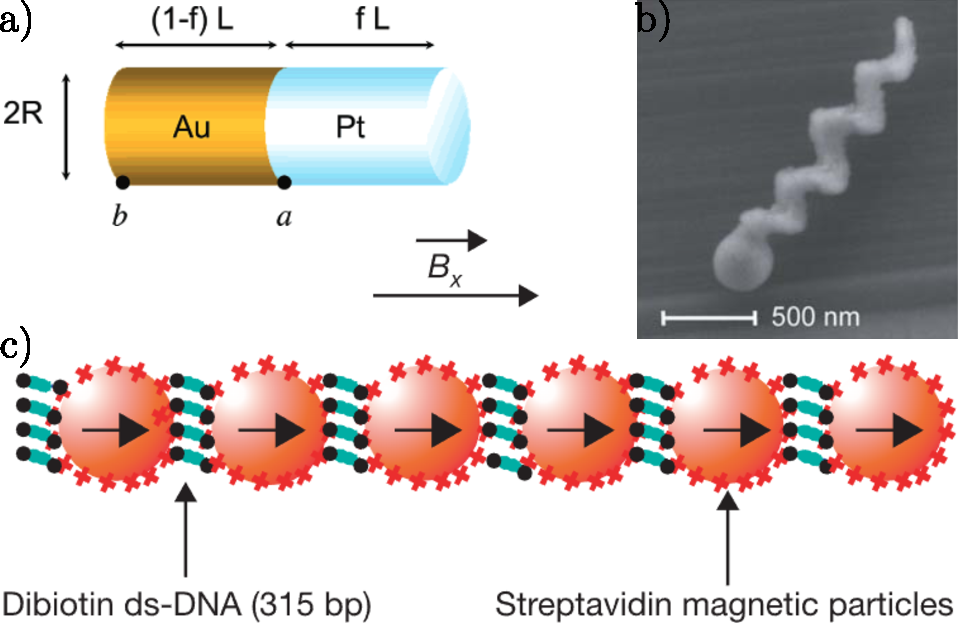
\includegraphics[width=0.95\textwidth]{figures/artificialExamples.pdf}
  \end{center}
  \caption[Artificail microswimmers]{\textbf{Panel 1)} shows the configuration of nanorods of Gold (Au) and Platinum (Pt), obtained from~\cite{paxton2004catalytic}. \textbf{Panel 2)} Shows a Silicon Dioxide nan rod, obtained from~\cite{ghosh2009controlled}.\textbf{Panel 3)} shows a chain of red blood cells linked with superparamagnetic filaments, obtained from~\cite{dreyfus2005microscopic}.}\label{fig:artificialexamples}
\end{figure}


However Howse et al. (2007) established the experimental basis for active Brownian particle dynamics by studying self-motile colloidal particles that use chemical reactions catalyzed on their surface to achieve autonomous propulsion. They demonstrated that at short times, these particles exhibit substantial directed motion with velocity dependent on fuel concentration, while at longer times, the motion transitions to a random walk with enhanced diffusion coefficients. This work provided a comprehensive experimental validation of the theoretical active Brownian particle model and established the standard mathematical framework for describing such systems through stochastic differential equations~\cite{howse2007self, palacci2010sedimentation}. These were done by coating polystyrene shperes with a layer of platinum, the same process as the plates and the nanorods, which will be the responsible of the propulsion method, nontheless, this in not inherently of the particle's shape, there have been assymetric artificial particles with an \textit{L} shape that undergoes the same behavior~\cite{kummel2013circular}.

Figure~\ref{fig:msddifferentvelocities} helps visualize how  the motion varies according to their velocity. When the average velocity is zero, the linear behavior of the MSD represents a diffusive behavior, whereas when it is different it is considered to be ballistic. 

\begin{figure}[h]
  \begin{center}
    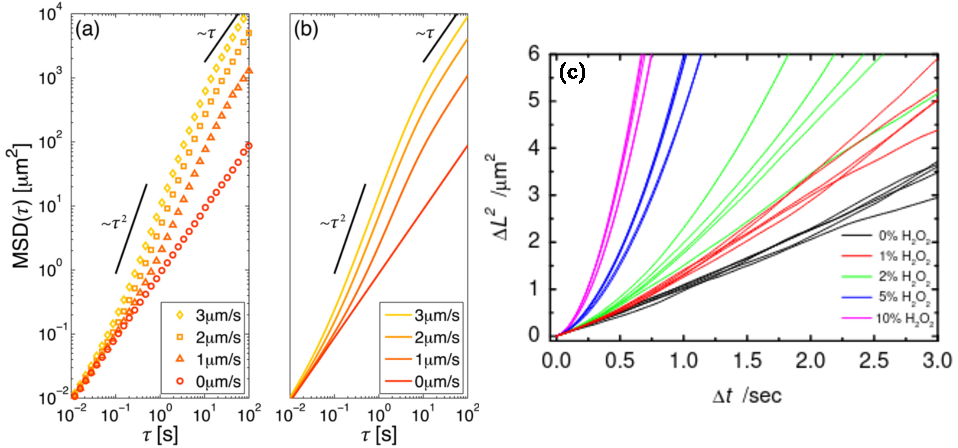
\includegraphics[width=0.85\textwidth]{figures/msdmicroscopicagents.pdf}
  \end{center}
  \caption[MSD for brownian particles]{MSD for brownian particles with different velocites. \textbf{Panel a)} shows the result from simulations. \textbf{Panel b)} shows the theoretical calculation, obtained from~\cite{volpe2014simulation}. \textbf{Panel c)} MSD for different velocities of polystyren spheres for different concentrations of Hydrogen Peroxide, obtained from~\cite{howse2007self}.}\label{fig:msddifferentvelocities}
\end{figure}

Tierno et al. (2008) proposed a new mechanism where two linked paramagnetic colloidal particles of different sizes, need no deformation for propulsion~\cite{tierno2008controlled}. Their setup consists of colloids dispersed in water above a flat glass plate in the presence of a precessing magnetic field parallel to the plate. Here, the plate plays an important role for the rotating colloids, due to the dynamics it has when particles are near a boundary. When the smaller one is near the glass, the viscosity increases, resulting in lateral translation of the small colloid.


Based on the premise of biomedical purposes, Ghosh et al. (2009) proposed a system where helical screw nano propellers' control is so precise that it can be manipulated with a tolerance of microns~\cite{ghosh2009controlled}. Their size is approximately 200-300 nm, making them ideal for navigating confined spaces inside and not being intrusive. They are driven by a magnetic field. Half of the helices are covered with cobalt, which has ferromagnetic properties, and then placed between two electromagnetic poles with a homogeneous precessing magnetic field, making the magnetic moment align with their long axis. Since the ferromagnetic part has a natural magnetic moment, it aligns with the external field, causing it to rotate along the helix. For each rotation, the particle moves either forward or backward, depending on certain values of the helix's geometry. 

\subsection{Natural Systems}

We note how researchers have developed numerous strategies to achieve what was already accomplished by nature over a long period. In this section, we will present some examples of biological agents that inspired this thesis.

 In a research by Corkidi et al. (2008) spermatozoa behavior was studied in a 3-dimensions space mimicking their real environment in searh for eggs, what they found was a helical trajectory, shown in Figure~\ref{fig:corkidiexperiment}, being a pretty similar response, and obtaining a non-space dependant behavior~\cite{corkidi2008tracking}. 

\begin{figure}[h]
  \begin{center}
    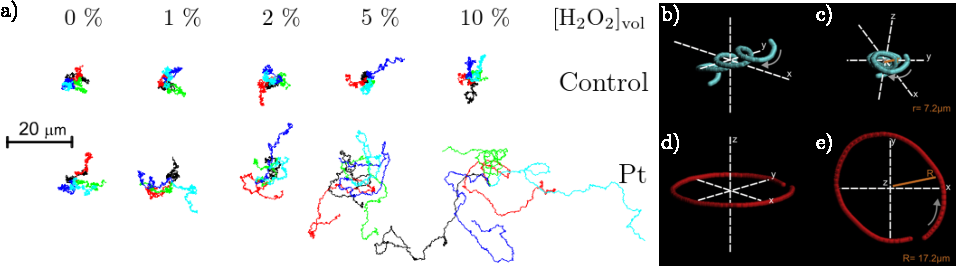
\includegraphics[width=0.90\textwidth]{figures/randomwalk.pdf}
  \end{center}
  \caption[Random Walk for active brownian particles.]{Trajectories of polystyren platinum layered sphere particles for different peroxide consentrations, obtained from~\cite{howse2007self}.Trajectory of the spermatozoa for \textbf{a,c} free space, and \textbf{b, d} confined 2-dimension space. Obtained from~\cite{corkidi2008tracking}.}\label{fig:corkidiexperiment}
\end{figure}



It seems we cannot avoid randomness even for active particles, in a regime where viscous forces are predominant, a little symmetry breaking noise that perturbs the direction of the particle can make the origin of a random walk, but nature, as always, has evolved elegant solutions to this challenge through various biological mechanisms. A prime example is E. coli, which employs helical flagella that can rotate both clockwise and counterclockwise, generating two distinct types of motion that researchers have termed "run"—swimming in a straight line—and "tumble"—rotation in a random direction. This behavior also depends on the medium's viscosity and random fluctuations~\cite{kumar2010physics}. The way E. coli achieves a "run" state is due to their flagella which has two different motions for its power and recovery strokes, simulating those of a human breast strokes, although a tumble state is unavoidable, it is a great opportunity to harness the directed motion of the particle and see if it is possible to obtain work of it. 


Marine bacteria are another example of an organic microswimmer; this can obtain individual speeds ten times faster than that of E. Coli (40 $\mu m s^{-1}$)~\cite{mitchell1995long, lowe1987rapid}. Marine bacteria have a similar mechanism as E. Coli, responding to amino acids utilising a run and reverse motion, different from the run and tumble, allowing them to stop and reverse their directon, making it more efficient reaction~\cite{barbara2003marine}. However, since this bacterium is often found in the ocean, where its nutrients are constantly in motion, a study by Barbara et al. (2002) aimed to investigate how it would react to obtain its nutrients~\cite{barbara2003bacterial}. Interestingly, thanks to the motion system, marine bacteria were able to turn multiple times in the direction of the nutrients, thereby tracking them unequivocally.

Another remarkable example of biologically active matter is the green alga \textit{Chlamydomonas reinhardtii}. This unicellular microorganism swims using two anterior flagella that beat in a breaststroke-like motion, propelling the cell forward through the water. Unlike bacteria, which rotate their helical flagella, \textit{Chlamydomonas} relies on the coordinated motion of paired flagella, leading to straight swimming when both are synchronized and to turning when the coordination is lost~\cite{goldstein2015green}. Because of this, \textit{Chlamydomonas} is often used as a model organism to understand how eukaryotic cells achieve motility at low Reynolds number.

Another type of biological microswimmer is found in protozoa such as \textit{Paramecium}. These ciliates are covered with thousands of cilia that beat in a coordinated manner, producing smooth gliding motion through viscous fluids~\cite{zhang2015paramecia}. Cilia not only enable propulsion but also allow \textit{Paramecium} to sense and respond to chemical gradients in their environment, demonstrating an early form of mechanosensory feedback in microswimmers.


Sometimes, bacteria exhibit such complex collective behavior that a new term was needed to describe it: \textit{liquid crystals}. This phenomenon usually appears in systems of elongated bacteria, where their shape and mutual interactions make the whole sample behave as something between a solid and a liquid. This intermediate state is what gives rise to the name \textit{liquid crystal}. These systems show characteristic features such as local orientation—resulting from the elongated shape of the cells, which allows this property to be measured—and the presence of topological defects, among others~\cite{decamp2015orientational}. There has been attempts to create artificial liquid crystals that mimic the biological ones. Sokolov \textit{et al.} (2025) done exactly that, with disodium cromoglycate, controlled by an acoustic field~\cite{sokolov2025synthetic}.

At a different scale, immune system cells, such as neutrophils, also display active motility, although they crawl rather than swim. Neutrophils move by extending actin-rich protrusions (lamellipodia) and contracting their cell body, enabling them to pursue pathogens in tissues~\cite{friedl2004collective}. While their propulsion mechanism differs from that of flagellated or ciliated organisms, neutrophils still exemplify how living systems consume energy internally to generate directed motion.

These diverse biological strategies demonstrate how nature has evolved multiple solutions to achieve motion in environments dominated by viscous forces. Each of these mechanisms—flagellar beating in algae, ciliary coordination in protozoa, or actin-driven crawling in immune cells—highlights the central role of active matter principles in biology. But, is their locomotion enough to produce work?

\section{Obtaining Work from Active Matter}

A fundamental question in active matter research is whether the continuous energy consumption and motion of biological microswimmers can be harnessed to perform useful work. In nature, molecular motors such as kinesin, dynein, and myosin already accomplish this inside cells, driving processes like vesicle transport, muscle contraction, and chromosome segregation. Inspired by these nanoscale examples, researchers have investigated whether intact organisms at the microscale can be used as biological engines outside their natural environments~\cite{schliwa2003molecular}.

One particularly illustrative example comes from the work of Weibel et al. (2005), who introduced the concept of \textit{``microoxen''} --- motile cells of the green alga \textit{Chlamydomonas reinhardtii}~\cite{weibel2005microoxen}. In their study, the authors exploited the flagellar beating of \textit{Chlamydomonas} to transport microscale loads such as polystyrene beads. By chemically attaching the beads to the cell wall, these algae were able to carry particles 1--6 µm in diameter without significantly reducing their swimming velocity (100–200 µm/s, similar to unmodified cells). 

An important feature of this work was the ability to control and manipulate the cells. Because \textit{Chlamydomonas} exhibits positive and negative phototaxis~\cite{bennett2015steering}, its direction of motion could be guided in microfluidic channels by alternating visible light sources. This allowed them to steer cargo-carrying cells back and forth repeatedly over distances of up to 20~cm. Moreover, by including a \textit{photocleavable chemical linker} between the load and the cell surface, they enabled the controlled release of particles using UV light, allowing cells to pick up, transport, and drop off cargo on demand.

This study highlights served as inspiration for using living active matter to perform mechanical work. On one hand, it demonstrates that whole microorganisms can act as microscopic carriers, and self-sustaining energy supply. On the other hand, it also underscores practical limitations: maintaining living cells, and preventing adhesion to surfaces.

 Qin et al. (2007) attempted to harness the dynamics of the decomposition of previously studied hydrogen peroxide, but rather than creating a system of linear motion, they employed it in a different manner. It is a similar approach as the nanorods, that use stripes of Pt and Au, this time they use a small surface, ressembling a path in one part of the rod, this configuration makes the release of oxygen bubbles in a lateral being capable of producing torque on the rod and therefore making it spin, thanks to this, they were able to create a nanorotor~\cite{qin2007rational}. However, we can argue that they are not harnessing the behavior of active matter to create work, but rather making active matter behave a certain way.

 \begin{figure}[h]
  \begin{center}
    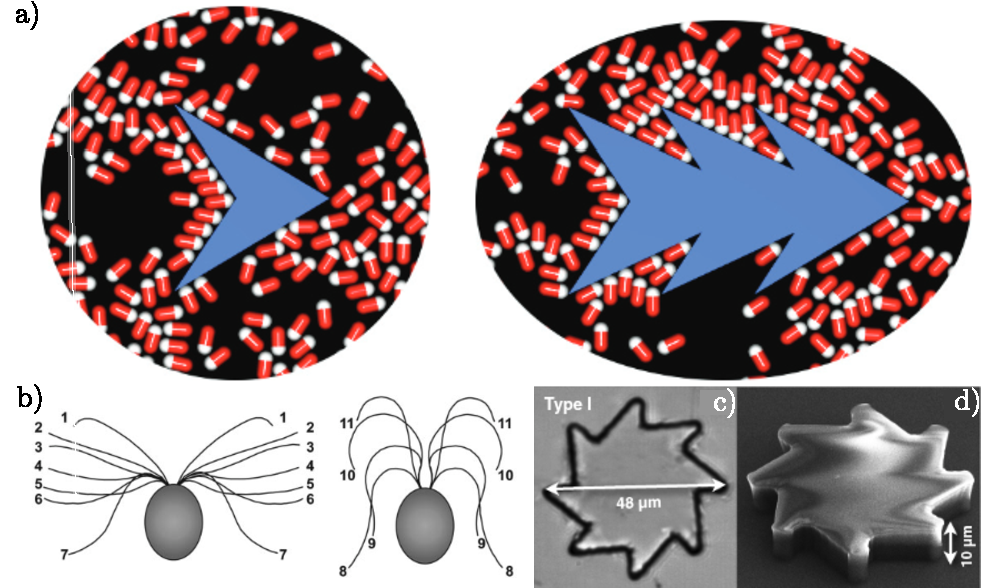
\includegraphics[width=0.95\textwidth]{figures/harnessWork.pdf}
  \end{center}
  \caption[Experiments that harness bacteria motility.]{Expermients that harness bacteria motility. \textbf{Panel 1)} shows how the bacteria accumulates in the concave sections of the shuttle, finally aligning parallelly, obtained from~\cite{angelani2010geometrically}. \textbf{Panel 2} drawing of Chlamydomonas reinhardtii's movement, obtained from~\cite{weibel2005microoxen}. \textbf{Panel 3) - 4)} shows an example of ratchet used in experiments, made by lithography, obtained from~\cite{di2010bacterial}.}\label{fig:harnesswork}
\end{figure}

Another novel demonstration of obtaining work from active matter was presented by Hiratsuka et al. (2006), who developed a microrotary motor powered by the gliding bacterium \textit{Mycoplasma mobile}~\cite{hiratsuka2006microrotary}. Unlike flagellated swimmers \textit{E. coli} or \textit{Chlamydomonas}, \textit{M. mobile} moves by gliding over solid surfaces at speeds of 2–5 µm/s, using sialic proteins in the surface of the track. The authors harnessed this motility by integrating living cells into lithographically fabricated microdevices.

Their microrotary motor consisted of a circular silicon track, into which \textit{M. mobile} cells were guided asymmetrically so that the majority moved in a unidirectional loop. A 20 µm silicon dioxide rotor with protrusions that fit into the circular track was then docked, and cells were chemically linked to its surface via biotin–streptavidin interactions. As the bacteria glided along the track, they pulled the rotor, producing unidirectional rotation at rates of 1.5–2.6 revolutions per minute (rpm). The torque generated by individual cells was estimated to be $2$–$5\times10^{-16}$ N·m, sufficient to overcome viscous drag at the microscale.

This work represents a successful integration of living motile cells with inorganic micromachinery, demonstrating that whole microorganisms can be harnessed to drive artificial devices. 


Angelani et al. (2010) noticed how asymmetric geometry can be used to harness the randomness of particles to obtain work from them. Using numerical simulations, they mimicked elongated motile bacteria, and the object to move consisted of an arrow-shaped structure with a varying number of teeth, ranging from 2 to 8. They saw that some particles get trapped between the spaces of the teeth, aligning themselves, making it possible to push the \textit{shuttle}, and due to dynamics, they eventually get unstuck and return to swim free in the solution. The simulations were performed in 2 dimensions, where bacteria were able to push the object~\cite{angelani2010geometrically}.

Beyond the use of single microorganisms as engines, researchers have also looked at how collective active matter might be used to produce work. Thampi et al. (2016) showed in simulations that dense active fluids—like bacterial suspensions or mixtures of microtubules with motor proteins—can display mesoscale turbulence that can be rectified to move micromachines~\cite{thampi2016active}.

In their setup, a square array of symmetric microrotors was placed inside an active nematic fluid. Although the rotors were geometrically identical, the system broke symmetry on its own: neighboring discs settled into an alternating spin pattern, rotating in opposite directions. In this way, disordered turbulent flows were turned into a regular and steady source of rotation. The extent and stability of the rotation depended on rotor size and spacing, with the best results when the separation was comparable to the natural vortex size of the active turbulence.

This study is useful here for two reasons. First, it shows that work can be obtained from active turbulence without introducing asymmetry or applying external fields. Second, it illustrates how geometry and confinement help stabilize active flows—ideas that will be relevant again in this thesis when we study colloids and ratchet systems under external driving.

A central question in active matter is how to harness the continuous energy consumption of self-propelled agents to perform useful work. Inside cells, proteins such as kinesin and dynein already fulfill this role at the nanoscale, but the prospect of exploiting entire microorganisms as microscopic engines is especially appealing. Early studies demonstrated that bacteria could be attached to synthetic objects and used to propel them forward~\cite{weibel2005microoxen, hiratsuka2006microrotary}. The resulting motion, however, was generally random.

A major advance came with the work of Di Leonardo et al. (2010), which served as inspiration for this thesis, showing that geometry alone can guide bacterial motion without the need for external fields~\cite{di2010bacterial}. In their experiments, sawtooth-shaped microgears with diameters of approximately 48~µm were immersed in dense suspensions of motile \textit{E. coli}. The bacteria accumulated and aligned at the concave corners of the gears, collectively exerting a torque that rotated the structures. At cell concentrations on the order of $10^{10}$~mL$^{-1}$, the gears achieved steady angular velocities of about 2~rpm. This behavior follows the mechanism described by Angelani et al. (2010), where cells become transiently trapped between the asymmetric teeth, pushing against the walls and generating directed motion~\cite{angelani2010geometrically}. 

Interestingly, the authors also tested different geometries. As expected, asymmetric rotors produced net rotation, while symmetric ones yielded zero average angular velocity, underscoring the importance of symmetry breaking in rectifying bacterial motion. 

This result demonstrates that combining bacterial activity with asymmetric boundaries can act as a ratchet, transforming random fluctuations into directed motion. The concept recalls the Feynman ratchet thought experiment, but here it is realized in a living system, powered solely by bacterial metabolism. Such bacterial ratchets not only provide fundamental insight into nonequilibrium statistical mechanics but also suggest potential applications in microfluidics, where pumps and mixers could operate autonomously without external energy inputs.


